\section{Background matematico}
Per poter discutere in modo rigoroso di tecniche di verifica del software,
è necessario introdurre alcuni concetti matematici di base relativi alla
teoria della computazione e alla logica formale.

\subsection{Set notation}
\begin{definizione}{Insieme}{set}
Un insieme (set) è una collezione di oggetti ben definiti e distinti.
La collezione stessa è considerata un oggetto a sé stante.

Dato un insieme $S$ è possibile dire che:
\begin{itemize}
    \item $s \in S$ significa che l'elemento $s$ appartiene all'insieme $S$.
    \item $S_{1}\subseteq S_{2}\triangleq\forall s\in S_{1}\Rightarrow s\in S_{2}$
    significa che l'insieme $S_{1}$ è un sottoinsieme di $S_{2}$ se ogni
    elemento di $S_{1}$ appartiene anche a $S_{2}$.
    \item $S_{1}\cup S_{2}=\{s|s\in S_{1}\vee s\in S_{2}\}$ è l'unione di
    due insiemi, ovvero l'insieme di tutti gli elementi che appartengono
    ad almeno uno dei due insiemi.
    \item $S_{1}\cap S_{2}=\{s|s\in S_{1}\wedge s\in S_{2}\}$ è l'intersezione
    di due insiemi, ovvero l'insieme di tutti gli elementi che appartengono
    ad entrambi gli insiemi.
\end{itemize}
\end{definizione}


\subsection{Partial order}

\begin{definizione}{Ordine parziale}{partial_order}

Un ordine parziale (partial order) è una relazione binaria $\sqsubseteq$ su un
insieme $X$ che soddisfa le seguenti proprietà:

\begin{itemize}
    \item Riflessività: $\forall x \in X \Rightarrow x \sqsubseteq x$, indica che ogni elemento è
    in relazione con se stesso.
    \item Anti-simmetria: $\forall x, y \in X, (x \sqsubseteq y \wedge y \sqsubseteq x)
    \Rightarrow x = y$, indica che se un elemento $x$ è in relazione con un altro
    elemento $y$ e viceversa, allora $x$ e $y$ sono lo stesso elemento.
    \item Transitività: $\forall x, y, z \in X, (x \sqsubseteq y \wedge y \sqsubseteq z)
    \Rightarrow x \sqsubseteq z$, indica che se un elemento $x$ è in relazione con un
    elemento $y$, e $y$ è in relazione con un elemento $z$, allora $x$ è in relazione
    con $z$.
\end{itemize}

\end{definizione}

\begin{esempio}{Esempio informale di ordine parziale su $\mathbb{Z}$}{es:informal_partial_order_z}

Informalmente è possibile considerare l'insieme dei numeri interi
$\mathbb{Z}$ con la relazione "minore o uguale di" ($\leq$) come un esempio di
ordine parziale. In questo caso è possibile verificare che:

\begin{itemize}
    \item Riflessività: Per ogni numero intero $i$, vale che $i \leq i$.
    \item Anti-simmetria: Se $i_1 \leq i_2$ e $i_2 \leq i_1$, allora $i_1 = i_2$.
    \item Transitività: Se $i_1 \leq i_2$ e $i_2 \leq i_3$, allora $i_1 \leq i_3$.
\end{itemize}

\end{esempio}

\subsection{Powerset}

\begin{definizione}{Insieme delle parti}{powerset}

Dato un insieme $S$, definito in \Cref{def:set}, l'insieme delle parti
(powerset) di $S$ è l'insieme di tutti i sottoinsiemi di $S$, ed è indicato
con $\mathcal{P}(S)$.

Dato un insieme $S$ con $|S| = n$ elementi è possibile determinare che l'insieme
delle parti di $S$ ha $|\mathcal{P}(S)| = 2^n$ elementi.

\end{definizione}

\begin{esempio}{Alcuni esempi di powerset}{es:powerset_examples}

    Dato l'insieme vuoto $\emptyset$, il suo powerset è:
    \[\mathcal{P}(\emptyset) = \{\emptyset\}\]
    ed ha $2^0 = 1$ elemento.

    Dato un insieme $X = \{a, b\}$, il suo powerset è:
    \[\mathcal{P}(X) = \{\emptyset, \{a\}, \{b\}, \{a, b\}\}\]
    ed ha $2^2 = 4$ elementi.

    Dato l'insieme $\mathbb{Z}$ dei numeri interi, il suo powerset è:
    \[\mathcal{P}(\mathbb{Z}) = \{\emptyset, \{\ldots, -2, -1, 0, 1, 2,
    \ldots\}, \{0\}, \{1, 2, 3\}, \ldots\}\]
    ed ha un numero infinito di elementi.

\end{esempio}

Dato un powerset è possibile definire un ordine parziale $\subseteq$ su di
esso e verificare che esso soddisfa le proprietà di un ordine parziale:

\begin{itemize}
    \item \textbf{Riflessività:} $\forall X_{1}\in \mathcal{P}(X). X_{1}\subseteq X_{1}$
    \item \textbf{Anti-simmetria:} $\forall X_{1},X_{2}\in\mathcal{P}(X).X_{1}\subseteq X_{2}\wedge X_{2}\subseteq X_{1}\Rightarrow X_{1}=X_{2}$
    \item \textbf{Transitività:} $\forall X_{1},X_{2},X_{3}\in\mathcal{P}(X).X_{1}\subseteq X_{2}\wedge X_{2}\subseteq X_{3}\Rightarrow X_{1}\subseteq X_{3}$
\end{itemize}


\begin{esercizio}{Inclusione inversa su powerset}{inverse_powerset_order}

L'inclusione inversa su un powerset $\mathcal{P}(X)$ è un ordine parziale?
Per verificare se $\supseteq$ è un ordine parziale su $\mathcal{P}(X)$,
è necessario verificare se soddisfa le tre proprietà di un ordine parziale.

\begin{itemize}
    \item \textbf{Riflessività:} $\forall X_1 \in \mathcal{P}(X) \Rightarrow
    X_1 \supseteq X_1$, indica che ogni insieme è sovrainsieme di se stesso.
    \item \textbf{Anti-simmetria:} $\forall X_1, X_2 \in \mathcal{P}(X),
    (X_1 \supseteq X_2 \wedge X_2 \supseteq X_1) \Rightarrow X_1 = X_2$,
    indica che se ogni elemento di $X_1$ è anche in $X_2$ e che ogni elemento di
    $X_2$ è anche in $X_1$, allora $X_1$ e $X_2$ sono lo stesso insieme.
    \item \textbf{Transitività:} $\forall X_1, X_2, X_3 \in \mathcal{P}(X),
    (X_1 \supseteq X_2 \wedge X_2 \supseteq X_3) \Rightarrow X_1 \supseteq X_3$,
    indica che se $X_1$ è un sovrainsieme di $X_2$, e $X_2$ è un sovrainsieme di
    $X_3$, allora $X_1$ è un sovrainsieme di $X_3$.
\end{itemize}

Poiché tutte e tre le proprietà sono soddisfatte, è possibile concludere che
l'inclusione inversa $\supseteq$ è un ordine parziale su il powerset
$\mathcal{P}(X)$. Quindi $\langle X, \supseteq \rangle$ è un poset.

\end{esercizio}

\subsection{Diagramma di Hasse}

Il diagramma di Hasse è una rappresentazione grafica di un poset.

Sia $X = \{ x, y, z \}$ un insieme (\Cref{def:set}), ed un poset $\langle X,
\sqsubseteq \rangle$ su di esso è possibile rappresentarlo tramite un diagramma
di Hasse dove una linea che connette $x$ e $y$ indica che:
\begin{itemize}
    \item $x \subseteq y$
    \item $\not\exists z \in X$ tale che $x \subseteq z \subseteq y$
\end{itemize}
È possibile trovare la presenza di più livelli nel diagramma di Hasse, dove
un elemento $x$ è posizionato più in alto di un elemento $y$ se $x$ è
``immediatamente maggiore'' di $y$.

\begin{nota}{Poset inverso}{nota:inverse_poset}
    Un poset inverso è un poset ottenuto invertendo la relazione di ordine
    di un poset originale.
    Graficamente, questo si traduce nel riflettere il diagramma di Hasse
    rispetto ad un asse orizzontale, ovvero ruotando di 180 gradi il diagramma.
\end{nota}

\begin{figure}[H]
    \centering
    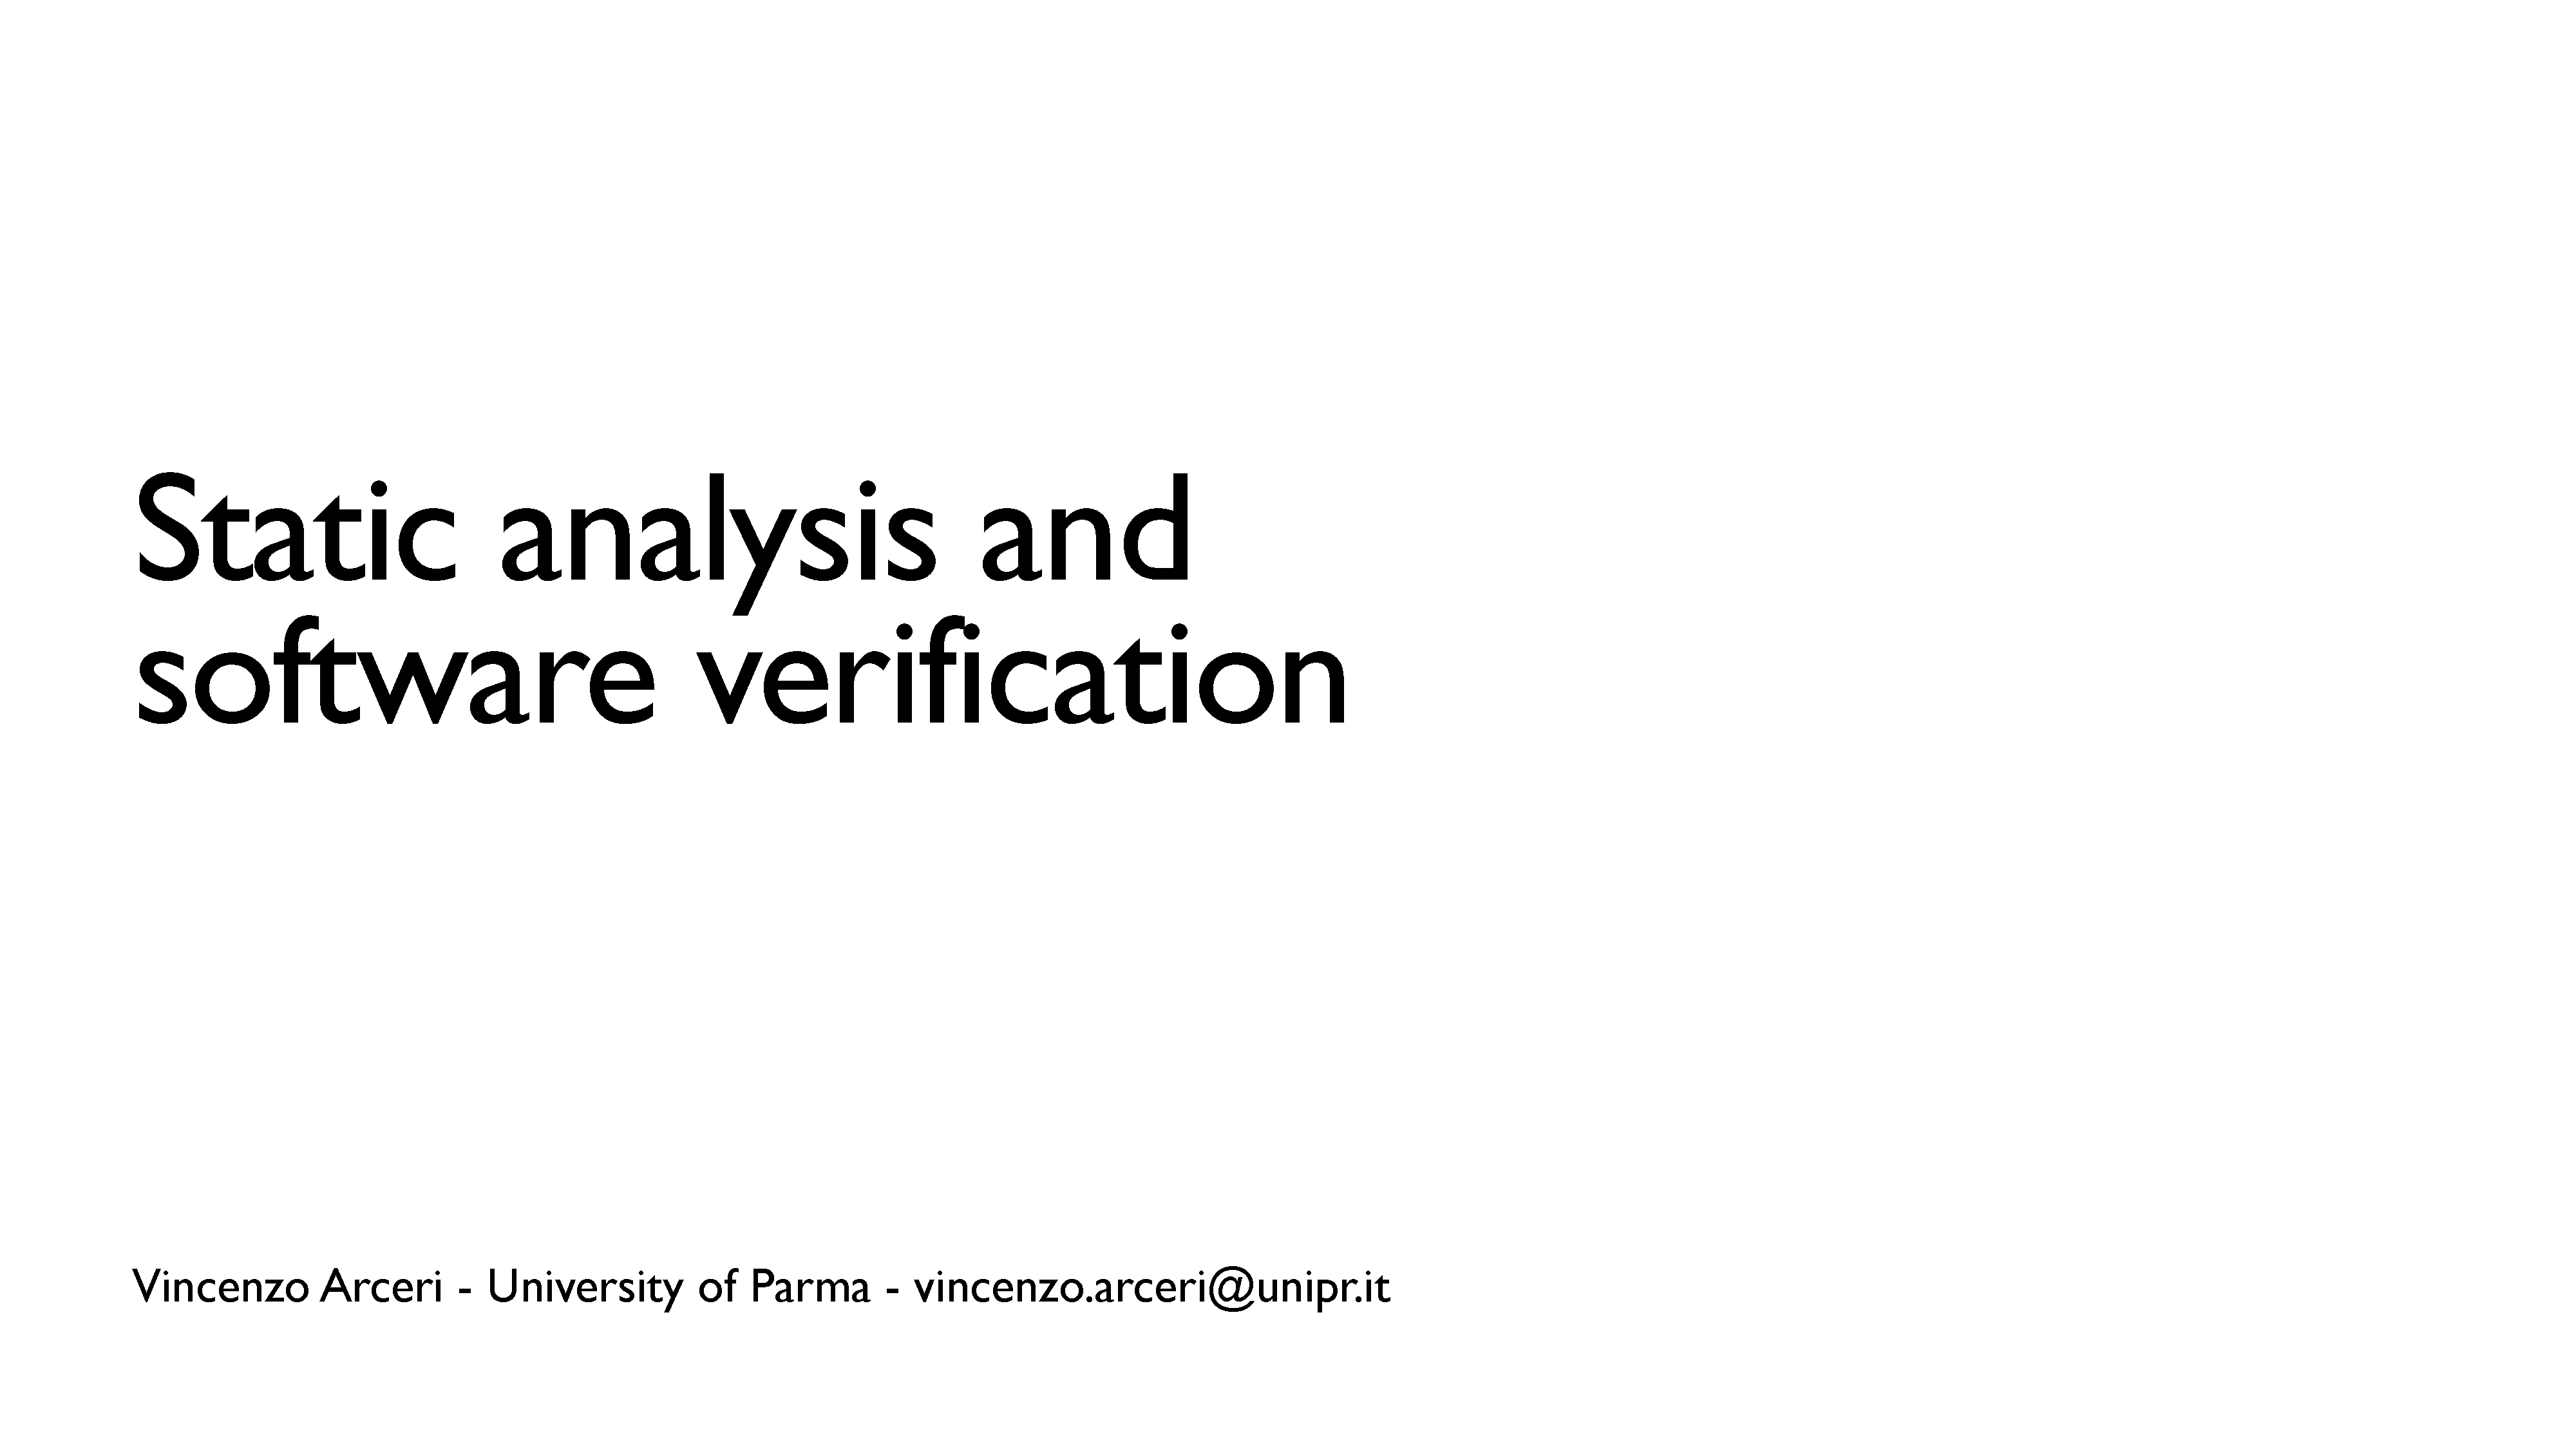
\includegraphics[width=0.8\textwidth]{images/th_02/01.png}
    \caption{L'immagine illustra un esempio di diagramma di Hasse per un poset
    e il suo poset inverso.}
    \label{fig:th_02_01}
\end{figure}

\subsection{Upper e lower bounds}

\begin{definizione}{Upper bound and least upper bound}{upper_bound}

Dato un poset $\langle X, \sqsubseteq \rangle$ e un sottoinsieme $Y \subseteq X$
è possibile dire che:
\begin{enumerate}
    \item $y \in X$ è un upperbound di $Y$ se $\forall y' \in Y, y' \sqsubseteq y$,
    ovvero se ogni elemento dell'insieme $Y$ è minore o uguale a $y$.
    \item $y$ è l'upperbound più piccolo tra tutti gli opperbound di $Y$, ovvero
    $\forall y' \in UB(Y). y \sqsubseteq y'$, dove $UB(Y)$ è l'insieme di
    tutti gli upperbound di $Y$.
\end{enumerate}

\end{definizione}

\begin{definizione}{Lower bound e greatest lower bound}{lower_bound}

Dato un poset $\langle X, \sqsubseteq \rangle$ e un sottoinsieme $Y \subseteq X$
è possibile dire che:
\begin{enumerate}
    \item $y \in X$ è un lowerbound di $Y$ se $\forall y' \in Y, y \sqsubseteq y'$,
    ovvero se ogni elemento dell'insieme $Y$ è maggiore o uguale a $y$.
    \item $y$ è il lowerbound più grande tra tutti i lowerbound di $Y$, ovvero
    $\forall y' \in LB(Y). y' \sqsubseteq y$, dove $LB(Y)$ è l'insieme di
    tutti i lowerbound di $Y$.
\end{enumerate}

\end{definizione}

\begin{esercizio}{Lub e glb su powerset}{lub_glb_powerset}
Dato il Poset $\langle \mathcal{P}(X), \subseteq \rangle$, e siano $S_{1},S_{2}\in \mathcal{P}(X)$:
\begin{enumerate}
    \item $S_{1}\cup S_{2}$ è l'estremo superiore (lub) di $\{S_{1},S_{2}\}$?
    \item $S_{1}\cap S_{2}$ è l'estremo inferiore (glb) di $\{S_{1},S_{2}\}$?
\end{enumerate}

\textbf{Soluzione esercizio 1}\\
$S_{1}\cup S_{2}$ è l'estremo superiore (lub) di $\{S_{1},S_{2}\}$?

Sia $L = S_1 \cup S_2$, che per essere lub deve soddisfare le condizioni elencate
in \Cref{def:upper_bound} punto 1 e 2.\\
Punto 1:\\
$S_1 \subseteq L$ e $S_2 \subseteq L$.\\
\\
Punto 2:\\
Sia $U$ un qualsiasi insieme tale che $S_1 \subseteq U$ e $S_2 \subseteq U$.
Allora $U$ deve per contenere gli elementi di $S_1$ e $S_2$ deve essere proprio
$(S_1 \cup S_2) \subseteq U$.\\
\\
\textbf{Soluzione esercizio 2}\\
$S_{1}\cap S_{2}$ è l'estremo inferiore (glb) di $\{S_{1},S_{2}\}$?
% TODO

\end{esercizio}
\subsection{Supremum e Infimum}

\begin{definizione}{Supremum}{supremum}

Dato un poset $\langle X, \sqsubseteq \rangle$ e un sottoinsieme $S \subseteq X$
il supremum (o least upper bound) di $S$ è l'elemento più piccolo tra tutti gli
upper bound di $S$.

\end{definizione}

\begin{definizione}{Infimum}{infimum}

Dato un poset $\langle X, \sqsubseteq \rangle$ e un sottoinsieme $S \subseteq X$
l'infimum (o greatest lower bound) di $S$ è l'elemento più grande tra tutti i
lower bound di $S$.

\end{definizione}

\subsection{Proprietà di lub e glb}
\begin{proposizione}{Proprietà di lub e glb}{prop:lub_glb_properties}
Dato un poset $\langle X, \sqsubseteq \rangle$ è possibile definire:
\begin{itemize}
    \item $\sqcup $ come il lub su $X$.
    \item $\sqcap $ come il glb su $X$.
    \item se $\sqcup $ e $\sqcap $ esistono sono unici.
    \item $\sqcup X$ esiste se e solo se $X$ ha un elemento $\top$ ($\sqcup X = \top$).
    \item $\sqcap X$ esiste se e solo se $X$ ha un elemento $\bot$ ($\sqcap X = \bot$).
\end{itemize}
\end{proposizione}
\subsection{Lattice}

\begin{definizione}{Lattice}{lattice}
Dato un poset $\langle X, \sqsubseteq \rangle$, esso è un reticolo (lattice) se
soddisfa entrambe le seguenti proprietà:

\begin{itemize}
    \item $\forall x,y \in X, \exists x \sqcup y$, ovvero per ogni coppia di elementi
    qualsiasi di $X$ deve esistere il loro lub.
    Un poset che soddisfa questa proprietà è detto ``join semi lattice''.
    \item $\forall x,y \in X, \exists x \sqcap y$, ovvero per ogni coppia di elementi
    qualsiasi di $X$ deve esistere il loro glb.
    Un poset che soddisfa questa proprietà è detto ``meet semi lattice''.
\end{itemize}

In un reticolo è presente la relazione d'ordine parziale $\sqsubseteq$ su due
elementi $x,y \in X$, ovvero $x \sqsubseteq y$ se e solo se:
\begin{itemize}
    \item $x \sqcup y = y$
    \item $x \sqcap y = x$
\end{itemize}

\begin{figure}[H]
    \centering
    \renewcommand{\arraystretch}{2.5}
    \begin{tabular}{c l}
        % --- Join semi-lattice ---
        \fbox{
        \begin{tikzpicture}[scale=0.8, transform shape]
            \node (T) at (0,0.8) {$\top$};
            \node (b) at (-0.5,0) {$b$};
            \node (c) at (0.5,0) {$c$};
            \draw (b) -- (T);
            \draw (c) -- (T);
        \end{tikzpicture}
        } & \textbf{Join semi-lattice} \\

        % --- Meet semi-lattice ---
        \fbox{
        \begin{tikzpicture}[scale=0.8, transform shape]
            \node (b) at (-0.5,0.8) {$b$};
            \node (c) at (0.5,0.8) {$c$};
            \node (bot) at (0,0) {$\bot$};
            \draw (bot) -- (b);
            \draw (bot) -- (c);
        \end{tikzpicture}
        } & \textbf{Meet semi-lattice} \\

        % --- Lattice ---
        \fbox{
        \begin{tikzpicture}[scale=0.8, transform shape]
            \node (T) at (0,1.6) {$\top$};
            \node (b) at (-0.5,0.8) {$b$};
            \node (c) at (0.5,0.8) {$c$};
            \node (bot) at (0,0) {$\bot$};
            \draw (bot) -- (b) -- (T);
            \draw (bot) -- (c) -- (T);
        \end{tikzpicture}
        } & \textbf{Lattice} \\
    \end{tabular}
    \caption{Rappresentazione grafica di Join semi-lattice, Meet semi-lattice e Lattice.}
    \label{fig:lattice_types}
\end{figure}

\end{definizione}

\subsection{Set lattice}

\begin{definizione}{Set lattice}{set_lattice}
Le operazioni insiemistiche definiscono una struttura di reticolo.
Dato il poset $\langle \mathcal{P}(X), \subseteq \rangle$, esso forma un
reticolo rispetto alle operazioni di unione ($\cup$) e intersezione
($\cap$), denotato come:
\[
\langle \mathcal{P}(X), \subseteq, \cup, \cap \rangle
\]

Se l'insieme $X$ è finito, allora il reticolo ha altezza finita.

\begin{figure}[H]
    \centering
    \includegraphics[width=0.4\textwidth]{images/th_02/02.png}
    \caption{L'immagine illustra un esempio di reticolo su un poset finito.}
    \label{fig:th_02_02}
\end{figure}

\end{definizione}

\begin{nota}{Top e Bottom nei reticoli}{set_lattice_top_bot}
Un reticolo non possiede necessariamente un elemento Top ($\top$) o
un elemento Bottom ($\bot$).
Ad esempio, il reticolo $\langle \mathbb{Z}, \leq, \max, \min \rangle$ non
ha né un elemento massimo né un elemento minimo, poiché l'insieme dei numeri
interi è illimitato in entrambe le direzioni.

\begin{figure}[H]
    \centering
    \includegraphics[width=0.8\textwidth]{images/th_02/03.png}
    \caption{L'immagine illustra il reticolo su $\mathbb{Z}$, privo di
    elementi top e bottom.}
    \label{fig:th_02_03}
\end{figure}

\end{nota}

\subsection{Complete lattice}

\begin{definizione}{Complete lattice}{complete_lattice}

Un reticolo $\langle X, \sqsubseteq, \sqcup, \sqcap \rangle$ è detto completo se:
\begin{itemize}
    \item Ogni sottoinsieme $Y \subseteq X$ ha un lub in $X$.
    \item È presente un elemento bottom $\bot$ in $X$.
\end{itemize}

\end{definizione}

\begin{esempio}{Esempi di lattice completo e non completo}{es:complete_lattice_example}

Considerando l'insieme dei numeri interi $\mathbb{Z}$ con la relazione
"minore o uguale di" ($\leq$), si può osservare che
\[
\langle \mathbb{Z}, \leq, \max, \min \rangle
\]
è un reticolo ma non è completo. Infatti, non esiste un elemento top
($\top$) in $\mathbb{Z}$, poiché non esiste un numero intero massimo.

Se all'insieme dei numeri interi si aggiungono gli elementi
$+\infty$ e $-\infty$, si ottiene l'insieme esteso
$\mathbb{Z} \cup \{+\infty, -\infty\}$. In questo caso, il reticolo
\[\langle \mathbb{Z} \cup \{+\infty, -\infty\}, \leq, \max, \min \rangle\]
diventa un reticolo completo, poiché ora esistono sia un elemento top
($+\infty$) che un elemento bottom ($-\infty$).

\begin{figure}[H]
    \centering
    \includegraphics[width=0.8\textwidth]{images/th_02/04.png}
    \caption{L'immagine illustra il reticolo su $\mathbb{Z} \cup \{+\infty, -\infty\}$.}
    \label{fig:th_02_04}
\end{figure}

\end{esempio}

\begin{proposizione}{Proprietà di un reticolo completo}{complete_lattice_properties}

Un reticolo completo possiede le seguenti proprietà:
\begin{itemize}
    \item reticolo completo $\langle X, \sqsubseteq, \sqcup, \sqcap \rangle$ ha un
    elemento top $\top$ e un elemento bottom $\bot$ e si denota come
    \[\langle X, \sqsubseteq, \top, \bot, \sqcup, \sqcap \rangle\]
    \item I reticoli finiti sono completi.
    \item $\sqcup$ induce $\sqcap : \sqcap S = \sqcup \{y | \forall x \in S . y \sqsubseteq x\}$
    \item $\sqcap$ induce $\sqcup : \sqcup S = \sqcap \{y | \forall x \in S . x \sqsubseteq y\}$
\end{itemize}

\end{proposizione}

\subsection{Relations}

\begin{definizione}{Prodotto cartesiano}{cartesian_product}
Dati due insiemi(\Cref{def:set}) $X$ e $Y$, il loro prodotto cartesiano $X \times Y$ è
l'insieme di tutte le possibili coppie ordinate $(x, y)$ dove il primo
elemento appartiene a $X$ e il secondo a $Y$ .
\[
X \times Y = \{ (x, y) \mid x \in X \land y \in Y \}
\]
\end{definizione}

\begin{definizione}{Relazione}{relation}
Una relazione $R$ tra due insiemi $X$ e $Y$ è definita come un sottoinsieme
del loro prodotto cartesiano (\Cref{def:cartesian_product}):
\[
R \subseteq X \times Y
\]
\end{definizione}

\begin{nota}{Notazione per le relazioni}{nota:relation_notation}
Dato una relazione $R \subseteq X \times Y$, è possibile indicare che
un elemento $x \in X$ è in relazione con un elemento $y \in Y$ tramite due
notazioni:
\begin{itemize}
    \item $(x, y) \in R$, ovvero tramite relazione insiemistica.
    \item $x \; R \; y$, ovvero tramite notazione infissa.
\end{itemize}

\end{nota}

\begin{nota}{Ordine parziale come relazione}{nota:partial_order_as_relation}
Un ordine parziale $\sqsubseteq$ (\Cref{def:partial_order}) è un caso
particolare di relazione definita sullo stesso insieme $X$.
Formalmente, $\sqsubseteq$ è un sottoinsieme del prodotto cartesiano
$X \times X$ ($\sqsubseteq \subseteq X \times X$).
A differenza di una relazione generica, l'ordine parziale deve soddisfare le
proprietà di riflessività, anti-simmetria e transitività (\Cref{def:partial_order}).
\end{nota}

\subsection{Functions (or maps)}

Le funzioni (functions), sono un tipo particolare di relazione, e sono
fondamentali per rioscire a modellare gli stati di un programma.

\begin{definizione}{Funzione}{function}

    Una funzione $f$ tra due insiemi $X$ e $Y$ è un particolare tipo di
relazione $R \subseteq X \times Y$ che soddisfa la proprietà di
unicità dell'immagine.

Formalmente, per ogni elemento $x$ nel dominio, esiste al massimo un
elemento $y$ nel codominio tale che $(x,y) \in f$:
\[
\forall (x, y) \in f, \nexists (x', y') \in f . (x = x' \land y \neq y')
\]
Una funzione è definita al massimo una volta su un dato input.
\end{definizione}

\begin{esempio}{Cerchio su un piano cartesiano}{es:circle_not_function}

    Un cerchio su un piano cartesiano non rappresenta una funzione, poiché
    un singolo valore di $x$ può essere associato a due valori distinti di
    $y$ (uno sopra l'asse $x$ e uno sotto). Questo viola la proprietà di
    unicità dell'immagine definita per le funzioni.

\end{esempio}

\begin{nota}{Non tutte le relazioni sono funzioni}{nota:rel_vs_func}
Un ordine parziale (\Cref{def:partial_order}) non è generalmente una funzione,
poiché un elemento può essere minore o uguale a molti altri elementi
(uno-a-molti).
\end{nota}


\begin{definizione}{Notazione delle funzioni}{func_notation}
Dato $f: X \to Y$, dove $X$ è il dominio e $Y$ è il codominio:
\begin{itemize}
    \item Notazione estensionale: Una funzione definita su punti specifici si scrive come:
    \[ f = [x_0 \mapsto y_0, x_1 \mapsto y_1, \dots, x_n \mapsto y_n] \]
    che è equivalente all'insieme di coppie $\{(x_0, y_0), (x_1, y_1), \dots, (x_n, y_n)\}$.
    
    \item Lambda notazione: Si utilizza $\lambda x . \textit{espressione}$ per
    definire una funzione anonima. Ad esempio $\lambda x . f(x) \equiv f$.
\end{itemize}
\end{definizione}

\subsubsection{Monotonia, Embedding e Isomorfismo}

Dati due posets $\langle X, \sqsubseteq_X \rangle$ e $\langle Y, \sqsubseteq_Y \rangle$,
e una funzione $f: X \to Y$, è possibile dire che:
\begin{itemize}
    \item La funzione $f$ è monotona se $x_1 \sqsubseteq_X x_2 \Rightarrow f(x_1) \sqsubseteq_Y f(x_2)$.
    \item La funzione $f$ è un embedding ordinato se $x_1 \sqsubseteq_X x_2 \iff f(x_1) \sqsubseteq_Y f(x_2)$.
    \item La funzione $f$ è un isomorfa se è un embedding ordinato ed è
    suriettiva, ovvero: $\forall y \in Y, \exists x \in X . f(x) = y$.
\end{itemize}

\begin{esempio}{Esempio di funzione monotona, embedding ordinato e suriettiva}{}
    Data $f: \langle \mathbb{Z}, \le \rangle \to \langle \mathbb{Z}, \le \rangle$,
    definita come $f(x) = x + 1$, è possibile osservare che:
    \begin{itemize}
        \item La funzione è monotona.
        \item La funzione è un embedding ordinato.
        \item La funzione è suriettiva.
    \end{itemize}

    \begin{figure}[H]
        \centering
        \includegraphics[width=0.8\textwidth]{images/th_02/05.png}
        \caption{L'immagine illustra la funzione $f(x) = x + 1$ come
        monotona, embedding ordinato e suriettiva.}
        \label{fig:th_02_05}
    \end{figure}
\end{esempio}


\begin{esempio}{Esempio di funzione monotona ma che non è un embedding}{}
    Data $f: \langle \mathcal{P}(\mathbb{Z}), \subseteq \rangle \to \langle \mathbb{Z}, \le \rangle$,
    definita come $f(X) = \max(X)$, è possibile osservare che:
    \begin{itemize}
        \item La funzione è monotona.
        \item La funzione non è un embedding.
    \end{itemize}

    \begin{figure}[H]
        \centering
        \includegraphics[width=0.8\textwidth]{images/th_02/06.png}
        \caption{L'immagine illustra la funzione $f(X) = \max(X)$ come
        monotona ma non un embedding.}
        \label{fig:th_02_06}
    \end{figure}
\end{esempio}


\subsubsection{Funzioni che preservano join e meet}

Dati due reticoli $\langle X, \sqsubseteq_X, \sqcup_X, \sqcap_X \rangle$ e
$\langle Y, \sqsubseteq_Y, \sqcup_Y, \sqcap_Y \rangle$, e una funzione
$f: X \to Y$, è possibile dire che:
\begin{itemize}
    \item La funzione $f$ preserva i join se $f(x_1 \sqcup_X x_2) =
    f(x_1) \sqcup_Y f(x_2)$.
    \item La funzione $f$ preserva i meet se $f(x_1 \sqcap_X x_2) =
    f(x_1) \sqcap_Y f(x_2)$.
\end{itemize}

\begin{nota}{Mantenimento della Monotonia}{nota:monotonicity_preservation}
Una funzione che preserva i join o i meet è monotona, ma una funzione che
è monotona non necessariamente preserva i join o i meet.
\end{nota}

\subsection{Chains}
\begin{definizione}{Catena}{chain}
Dato un poset $\langle X, \sqsubseteq \rangle$, una catena (chain) $S$ se
tutti gli elementi contenuti sono completamente ordinati, ovvero:
\[
\forall x,y \in S . x \sqsubseteq y \vee y \sqsubseteq x
\]
\end{definizione}

\begin{esempio}{Esempio di catena}{chain_example}
    Dato un poset $\langle \mathcal{P}(\mathbb{Z}), \subseteq \rangle$ con
    reticolo rappresentato nell'immagine sottostante (\ref{fig:th_02_07}),
    esempi di catene sono:
    \begin{itemize}
        \item $\{\emptyset\}$
        \item $\{\emptyset, \{0, 1\}\}$
        \item $\{\{0\}, \{-1, 0, 1\}\}$
    \end{itemize}

    \begin{figure}[H]
        \centering
        \includegraphics[width=0.5\textwidth]{images/th_02/07.png}
        \caption{L'immagine illustra un reticolo su $\mathcal{P}(\mathbb{Z})$.}
        \label{fig:th_02_07}
    \end{figure}
\end{esempio}

\subsubsection{Ascending Chain Condition (ACC)}

\begin{definizione}{Catena Ascendente}{ascending_chain}
Una catena ascendente è una sequenza di elementi $(l_n)_{n \in \mathbb{N}}$
indicizzata dai numeri naturali tali che:
\[
i \le j \implies l_i \sqsubseteq l_j
\]
Ovvero $l_0 \sqsubseteq l_1 \sqsubseteq l_2 \sqsubseteq \dots$.
\end{definizione}

\begin{definizione}{Ascending Chain Condition (ACC)}{acc}
Un poset soddisfa la Ascending Chain Condition (ACC) se ogni catena ascendente
infinita si stabilizza (non è strettamente crescente per sempre).

Matematicamente, una catena $(l_n)$ si stabilizza se:
\[
\exists k \ge 0 . \forall j \ge k . l_k = l_j
\]
Questo significa che, dopo un certo indice $k$, tutti gli elementi successivi
sono uguali a $l_k$ (il punto fisso della sequenza).
\end{definizione}

\begin{esempio}{Esempio di catena ascentente infinita non è stettamente crescente}{}
Un esempio di catena ascentente infinita non stettamente crescente è la seguente:
\[
 \exists k \ge 0 . \forall j \ge k . l_k = l_j
\]
Perché dopo un certo numero di passi $k$, tutti gli elementi successivi
della catena sono uguali a $l_k$. Ovvero la catena si stabilizza.
\end{esempio}

\subsection{Fixpoint}
